\documentclass{beamer}
\usepackage[english]{babel}
\usepackage[utf8]{inputenc, vietnam}

\mode<presentation> {

% The Beamer class comes with a number of default slide themes
% which change the colors and layouts of slides. Below this is a list
% of all the themes, uncomment each in turn to see what they look like.

%\usetheme{default}
%\usetheme{AnnArbor}
%\usetheme{Antibes}
%\usetheme{Bergen}
%\usetheme{Berkeley}
%\usetheme{Berlin}
%\usetheme{Boadilla}
%\usetheme{CambridgeUS}
%\usetheme{Copenhagen}
%\usetheme{Darmstadt}
%\usetheme{Dresden}
%\usetheme{Frankfurt}
%\usetheme{Goettingen}
%\usetheme{Hannover}
%\usetheme{Ilmenau}
%\usetheme{JuanLesPins}
%\usetheme{Luebeck}
\usetheme{Madrid}
%\usetheme{Malmoe}
%\usetheme{Marburg}
%\usetheme{Montpellier}
%\usetheme{PaloAlto}
%\usetheme{Pittsburgh}
%\usetheme{Rochester}
%\usetheme{Singapore}
%\usetheme{Szeged}
%\usetheme{Warsaw}

% As well as themes, the Beamer class has a number of color themes
% for any slide theme. Uncomment each of these in turn to see how it
% changes the colors of your current slide theme.

%\usecolortheme{albatross}
%\usecolortheme{beaver}
%\usecolortheme{beetle}
%\usecolortheme{crane}
%\usecolortheme{dolphin}
%\usecolortheme{dove}
%\usecolortheme{fly}
%\usecolortheme{lily}
%\usecolortheme{orchid}
%\usecolortheme{rose}
%\usecolortheme{seagull}
%\usecolortheme{seahorse}
%\usecolortheme{whale}
%\usecolortheme{wolverine}

%\setbeamertemplate{footline} % To remove the footer line in all slides uncomment this line
%\setbeamertemplate{footline}[page number] % To replace the footer line in all slides with a simple slide count uncomment this line

%\setbeamertemplate{navigation symbols}{} % To remove the navigation symbols from the bottom of all slides uncomment this line
}

\usepackage{graphicx} % Allows including images
\usepackage{booktabs} % Allows the use of \toprule, \midrule and \bottomrule in tables

%----------------------------------------------------------------------------------------
%	TITLE PAGE
%----------------------------------------------------------------------------------------

\title[Chuỗi thời gian PM10]{Mô hình hóa chuỗi thời gian quan trắc\\và phân tích nồng độ chất ô nhiễm không khí} % The short title appears at the bottom of every slide, the full title is only on the title page

\author[Nguyễn Ngọc Thuận]{Nguyễn Ngọc Thuận\\GVHD: TS. Nguyễn Văn Minh Mẫn} % Your name
\institute[] % Your institution as it will appear on the bottom of every slide, may be shorthand to save space
{
Đại học Bách Khoa, TP.HCM \\ % Your institution for the title page
}
\date{\today} % Date, can be changed to a custom date

\begin{document}
	
\begin{frame}
\titlepage 
\end{frame}

\begin{frame}{Nội dung}
\begin{enumerate}
\item Giới thiệu đề tài
\item Đối tượng và mục tiêu nghiên cứu
\item Phương pháp nghiên cứu
\item Kế hoạch triển khai
\item Nội dung dự kiến
\item Kết luận
\end{enumerate}
\end{frame}

\begin{frame}{Nội dung}
\begin{enumerate}
\item {\color{red}Giới thiệu đề tài}
\item Đối tượng và mục tiêu nghiên cứu
\item Phương pháp nghiên cứu
\item Kế hoạch triển khai
\item Nội dung dự kiến
\item Kết luận
\end{enumerate}
\end{frame}

\begin{frame}{PM10 (Particulate matter)}
Giới thiệu chất \textit{PM10 (Particulate matter)}
\begin{itemize}
\item Gồm những hạt bụi chất lỏng và chất rắn
\item Đường kính nhỏ hơn 10 \(\mu m\)
\item Có thể đi sâu vào bên trong phổi, gây ung thư
\item Là một trong những chất gây ô nhiễm không khí\\
 (QCVN 05:2013/BTNMT)
\end{itemize}
Vì vậy, ta có các trạm quan trắc chất PM10.
\end{frame}

\begin{frame}{Trạm quan trắc đặt ở vườn thú thành phố}
Thời gian hoạt động
\begin{itemize}
\item Ghi nhận 24 lần / ngày
\item Khoảng thời gian giữa 2 lần ghi kế tiếp là 1 tiếng.
\item Dữ liệu của mỗi lần ghi là
\begin{itemize}
\item {\color{blue}số thực không âm (\(\mu g / m^3\)) (giá trị hợp lệ)}
\item {\color{red}-9900}
\item {\color{red}giá trị rỗng}
\item {\color{red}MA}
\end{itemize}
\item Quan trắc từ 1:00 ngày 01/01/2003 \(\to\) 23:00 ngày 25/04/2004
\end{itemize}
\end{frame}

\begin{frame}{Tập dữ liệu}
Nồng độ chất PM10 quan trắc ở vườn thú thành phố
 vào ngày 02/01/2003.
\begin{figure}[!h]\centering
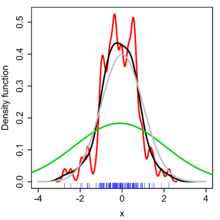
\includegraphics [scale=0.5] {220px-Comparison_of_1D_bandwidth_selectors.png}
\end{figure}
\end{frame}

\begin{frame}{Nêu bài toán}
Đề tài nghiên cứu cách lập mô hình nồng độ chất PM10
\begin{itemize}
\item Để dự báo nồng độ trong tương lai
\item Dùng dữ liệu chuỗi thời gian của trạm quan trắc ở vườn thú
\item Áp dụng lý thuyết chuỗi thời gian + thiết kế thí nghiệm
\item Hiện thực cách lập mô hình bằng máy tính
\end{itemize}
\begin{figure}[!h]\centering
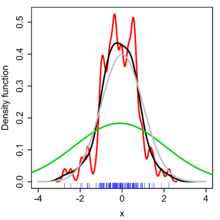
\includegraphics [scale=0.75] {220px-Comparison_of_1D_bandwidth_selectors.png}
\end{figure}
\end{frame}

\begin{frame}{Đóng góp của đề tài}
Tính thực tiễn: Đề xuất một mô hình nồng độ PM10
\begin{itemize}
\item Sẽ được kiểm chứng trên dữ liệu thật
\item Có thể dùng tham khảo khi lập mô hình các chất khí khác
\item Dùng để dự báo về môi trường
\end{itemize}
Tính khoa học: Kết hợp lý thuyết chuỗi thời gian +
 thiết kế thí nghiệm để mô hình hóa hiện tượng khi
 có nhiều nguồn ảnh hưởng.
\end{frame}

\begin{frame}{Các nghiên cứu liên quan}
\begin{itemize}
\item Các tài liệu ở mục tham khảo chưa tuyên bố
 có phương pháp lập mô hình tốt nhất
\item Phần mềm thống kê \(\mathcal{R}\) có hàm
 \textit{auto.arima} trong gói \textit{forecast}, tham số mặc định
 cho mô hình có phương sai là 428, khá lớn so với trung bình mẫu
 là 54.
\end{itemize}
\end{frame}

\begin{frame}{Nội dung}
\begin{enumerate}
\item Giới thiệu đề tài
\item {\color{red}Đối tượng và mục tiêu nghiên cứu}
\item Phương pháp nghiên cứu
\item Kế hoạch triển khai
\item Nội dung dự kiến
\item Kết luận
\end{enumerate}
\end{frame}

\begin{frame}{Mô hình hóa sự quan sát}
	\begin{itemize}
	\item Số lần quan sát: \(n\)
	\item Cho \(j = \overline{1, n}\): quan sát thứ \(j^{th}\) là một phép thử ngẫu nhiên, có
		\begin{itemize}
		\item Biến ngẫu nhiên \(X_j\) và giá trị ghi nhận \(x_j\),
		\item với \(X_j: \mathbb{R}^+ \to \mathbb{R}^+ \cup \{-1\}\),\\
		 trong đó \(-1\) để chỉ những giá trị không hợp lệ.
		\end{itemize}
	\end{itemize}
Như vậy, ta có \(2\) dãy
	\begin{itemize}
	\item \(\mathbf{X} = \{X_1, X_2, \ldots, X_n\}\)
	\item \(\mathbf{x} = \{x_1, x_2, \ldots, x_n\}\)
	\end{itemize}
\end{frame}

\begin{frame}{Mô hình hóa các yếu tố ảnh hưởng}
\begin{itemize}
\item \(A\): Yếu tố chỉ ngày - đêm, có 2 mức chọn
	\begin{itemize}
	\item 0: ngày (7:00 \(\to\) 18:00)
	\item 1: đêm
	\end{itemize}
\item \(B\): Yếu tố chỉ ngày làm việc - ngày cuối tuần, có 2 mức chọn
	\begin{itemize}
	\item 0: ngày làm việc (0:00 thứ hai \(\to\) 23:00 thứ sáu)
	\item 1: ngày cuối tuần
	\end{itemize}
\end{itemize}
\begin{table}
\centering

\begin{tabular}{|c|c|c|c|}
\hline
\textbf{Date} & \textbf{PM10 (\(\boldsymbol{\mu}\mathbf{g/m^3}\))} & \(\mathbf{A}\) & \(\mathbf{B}\) \\ \hline
1/1/2003 1:00 (Wed) & 87 & 1 & 0 \\ \hline
\vdots & \vdots & \vdots & \vdots \\ \hline
1/1/2003 7:00 (Wed) & 128 & 0 & 0 \\ \hline
\vdots & \vdots & \vdots & \vdots \\ \hline
1/4/2003 (Sat) & 118 & 1 & 1 \\ \hline
\vdots & \vdots & \vdots & \vdots \\ \hline
1/6/2003 (Mon) & 111 & 1 & 0 \\
\hline
\end{tabular}
\end{table}
\end{frame}

\begin{frame}{Ràng buộc trên tập dữ liệu}
\begin{itemize}
\item Chỉ dùng những đoạn dữ liệu có giá trị hợp lệ,
 không gián đoạn, thời gian quan sát hơn 30 ngày.
\item Các biến ngẫu nhiên có phương sai hữu hạn.
\end{itemize}
\end{frame}

\begin{frame}{Mục tiêu đề tài}
Kết quả cần đạt được
\begin{itemize}
\item Mô hình chuỗi thời gian nồng độ chất PM10 ở vườn thú, trong đó
	\begin{itemize}
	\item Sai số = giá trị quan sát - giá trị dự báo của mô hình
	\item Các sai số \(\sim N(0, \sigma^2)\)
	\end{itemize}
\item Sự phân tích các yếu tố ảnh hưởng
\item Mã lệnh thực thi trên phần mềm \(\mathcal{R}\)
\end{itemize}
\end{frame}

\begin{frame}{Nội dung}
\begin{enumerate}
\item Giới thiệu đề tài
\item Đối tượng và mục tiêu nghiên cứu
\item {\color{red}Phương pháp nghiên cứu}
\item Kế hoạch triển khai
\item Nội dung dự kiến
\item Kết luận
\end{enumerate}
\end{frame}

\begin{frame}{Lý thuyết chuỗi thời gian}
\begin{itemize}
\item Các khái niệm: chuỗi thời gian, quá trình ngẫu nhiên,
 quá trình ổn định, ước lượng giá trị trung bình, hiệp phương sai, hệ số tương quan.
\item Kiểm định quá trình ổn định
\item Chọn mô hình: ARMA(\(p, q\)), ARIMA(\(p, d, q\)).
\item Ướm mô hình: \textit{phương pháp ước lượng cơ may cực đại
 (maximum likelihood estimation)}
\item Kiểm định mô hình: \textit{kiểm định biên (test bounds)}, Ljung - Box,
 kiểm định sự phân phối chuẩn của các sai số \(\{e_1, \ldots, e_n\}\)
\item So sánh mô hình: tiêu chuẩn thông tin AIC, BIC.
\end{itemize}
\end{frame}

\begin{frame}{Lý thuyết thiết kế thí nghiệm}
\begin{itemize}
\item Các nguyên lý: lặp, ngẫu nhiên, phân khối.
\item Mô hình cộng tính và không cộng tính
\item Thiết kế nhân tố đầy đủ: \(2^m, 3^m\), phân tích phương sai, \ldots
\item Thêm yếu tố vào mô hình chuỗi thời gian. Ví dụ
\[X_t = a X_{t-1} + b A + \varepsilon_t.\]
\end{itemize}
\end{frame}

\begin{frame}{Đánh giá mô hình kết quả}
Phương pháp \textit{kiểm tra chéo bỏ một phần tử (leave-one-out cross-validation)}
\begin{enumerate}
\item Dùng \(n-1\) phần tử trong tập dữ liệu cỡ \(n\) \{\(x_1, \ldots, x_n\)\}
 để mô hình hóa
\item Dùng 1 phần tử còn lại để tính sai số
\item Tiến hành \(n\) lần bước 1 và 2, ta có tập sai số cỡ \(n\) \{\(e_1, \ldots, e_n\)\}
\item Đánh giá tập sai số khớp với sai số của mô hình.
\end{enumerate}
\end{frame}

\begin{frame}{Nội dung}
\begin{enumerate}
\item Giới thiệu đề tài
\item Đối tượng và mục tiêu nghiên cứu
\item Phương pháp nghiên cứu
\item {\color{red}Kế hoạch triển khai}
\item Nội dung dự kiến
\item Kết luận
\end{enumerate}
\end{frame}

\begin{frame}{Kế hoạch triển khai}
Đề tài thực hiện trong 20 tuần
\begin{table}
\centering
\begin{tabular}{|c|c|}
\hline
\textbf{Công việc} & \textbf{Thời gian (tuần)} \\ \hline
Đề xuất ý tưởng lập mô hình & 1 \\ \hline
Nghiên cứu mô hình ARMA(\(p, q\)) & 2 \\ \hline
Nghiên cứu mô hình ARIMA(\(p, d, q\)) & 2 \\ \hline
Tiêu chuẩn thông tin AIC, BIC & 3 \\ \hline
Lý thuyết thiết kế thí nghiệm & 2 \\ \hline
Đề xuất phương pháp lập mô hình & 1 \\ \hline
Cài đặt trên máy tính & 2 \\ \hline
Đánh giá, cải tiến & 3 \\ \hline
Viết báo cáo & 4 \\ \hline
\end{tabular}
\end{table}
\end{frame}

\begin{frame}{Nội dung}
\begin{enumerate}
\item Giới thiệu đề tài
\item Đối tượng và mục tiêu nghiên cứu
\item Phương pháp nghiên cứu
\item Kế hoạch triển khai
\item {\color{red}Nội dung dự kiến}
\item Kết luận
\end{enumerate}
\end{frame}

\begin{frame}{Nội dung chính dự kiến}
\begin{itemize}
\item Chương 1: Tổng quan nội dung luận văn.
	\begin{itemize}
	\item Mô tả tập dữ liệu
	\item Ý nghĩa đề tài
	\item Tóm tắt kết quả luận văn
	\end{itemize}
\item Chương 2: Cơ sở lý thuyết lập mô hình
	\begin{itemize}
	\item Mô hình hóa bài toán
	\item Các dạng mô hình WN(0, \(\sigma^2\)),
	AR(\(p\)), MA(\(q\)), ARMA(\(p, q\)), ARIMA(\(p, d, q\))
	\item Tiêu chuẩn thông tin AIC, BIC
	\end{itemize}
\item Chương 3: Hướng tiếp cận dùng lý thuyết thiết kế thí nghiệm
	\begin{itemize}
	\item Mô hình hóa các yếu tố ảnh hưởng
	\item Các nguyên lý thiết kế, dạng thiết kế  \(2^m, 3^m\)
	\end{itemize}
\item Chương 4: Đề xuất phương pháp lập mô hình.
	\begin{itemize}
	\item Áp dụng trên tập dữ liệu PM10
	\item Hiện thực trên máy tính
	\item Đánh giá kết quả
	\end{itemize}
\item Chương 5: Kết luận.
\item Phụ lục: Mã thực thi phương pháp trên \(\mathcal{R}\)
\end{itemize}
\end{frame}

\begin{frame}{Nội dung}
\begin{enumerate}
\item Giới thiệu đề tài
\item Đối tượng và mục tiêu nghiên cứu
\item Phương pháp nghiên cứu
\item Kế hoạch triển khai
\item Nội dung dự kiến
\item {\color{red}Kết luận}
\end{enumerate}
\end{frame}

\begin{frame}{Kết luận}
Xuất phát từ bài toán thực tiễn dự báo nồng độ PM10,
 đề tài bao gồm
\begin{itemize}
\item Nghiên cứu lập mô hình chuỗi thời gian
\item Phân tích các yếu tố ảnh hưởng
\item Hiện thực phương pháp trên máy tính
\item Kiểm chứng với tập dữ liệu ở vườn thú
\end{itemize}
\end{frame}

\begin{frame}{Tài liệu tham khảo}
\begin{thebibliography}{9}
\section*{Tài liệu nước ngoài}
\bibitem{Brockwell_intro}
	Brockwell, P. J. and Davis, R. A. (2002),
	\emph{Introduction to Time Series and Forecasting (2nd ed.)},
	Springer-Verlag, New York.
\bibitem{Brockwell_theory}
	Brockwell, P. J. and Davis, R. A. (2006),
	\emph{Time Series: Theory and Methods, (2nd ed.)},
	Springer.
\bibitem{Ruppert}
	Ruppert, D. (2011).
	\emph{Statistics and Data Analysis for Financial Engineering},
	Springer.
\section*{Tài liệu trong nước}
\bibitem{ManNguyen}
	Nguyễn V. M. Mẫn (2015),
	"Thống kê ứng dụng với ví dụ viết trên ngôn ngữ \(\mathcal{R}\)",
	\emph{SMA Workshop}, VNUHCM \& CTU, Việt Nam.
\section*{Website}
\bibitem{R}
	\emph{The Comprehensive R Archive Network}, truy cập ngày 20 tháng 5 năm 2015,
	địa chỉ \emph{http://cran.r-project.org/index.html}.
\end{thebibliography}

\end{frame}

\end{document}
